%%%%%%%%%%%%%%%%%%%%%%%%%%%%%%%%%%%%%%%%%%%%%%%%%%%%%%%%%%%%%%%%%%%%%%%%%%%%%%%%%%%%%%%%%%%
%%%%%%%%%%%%%%%%%%%%%%%%%%%%%%%%%%%%%% Preambule %%%%%%%%%%%%%%%%%%%%%%%%%%%%%%%%%%%%%%%%%
%%%%%%%%%%%%%%%%%%%%%%%%%%%%%%%%%%%%%%%%%%%%%%%%%%%%%%%%%%%%%%%%%%%%%%%%%%%%%%%%%%%%%%%%%%

\documentclass[a4paper, 12pt, leqno]{article}\usepackage[]{graphicx}\usepackage[]{color}
%% maxwidth is the original width if it is less than linewidth
%% otherwise use linewidth (to make sure the graphics do not exceed the margin)
\makeatletter
\def\maxwidth{ %
  \ifdim\Gin@nat@width>\linewidth
    \linewidth
  \else
    \Gin@nat@width
  \fi
}
\makeatother

\definecolor{fgcolor}{rgb}{0.345, 0.345, 0.345}
\newcommand{\hlnum}[1]{\textcolor[rgb]{0.686,0.059,0.569}{#1}}%
\newcommand{\hlstr}[1]{\textcolor[rgb]{0.192,0.494,0.8}{#1}}%
\newcommand{\hlcom}[1]{\textcolor[rgb]{0.678,0.584,0.686}{\textit{#1}}}%
\newcommand{\hlopt}[1]{\textcolor[rgb]{0,0,0}{#1}}%
\newcommand{\hlstd}[1]{\textcolor[rgb]{0.345,0.345,0.345}{#1}}%
\newcommand{\hlkwa}[1]{\textcolor[rgb]{0.161,0.373,0.58}{\textbf{#1}}}%
\newcommand{\hlkwb}[1]{\textcolor[rgb]{0.69,0.353,0.396}{#1}}%
\newcommand{\hlkwc}[1]{\textcolor[rgb]{0.333,0.667,0.333}{#1}}%
\newcommand{\hlkwd}[1]{\textcolor[rgb]{0.737,0.353,0.396}{\textbf{#1}}}%
\let\hlipl\hlkwb

\usepackage{framed}
\makeatletter
\newenvironment{kframe}{%
 \def\at@end@of@kframe{}%
 \ifinner\ifhmode%
  \def\at@end@of@kframe{\end{minipage}}%
  \begin{minipage}{\columnwidth}%
 \fi\fi%
 \def\FrameCommand##1{\hskip\@totalleftmargin \hskip-\fboxsep
 \colorbox{shadecolor}{##1}\hskip-\fboxsep
     % There is no \\@totalrightmargin, so:
     \hskip-\linewidth \hskip-\@totalleftmargin \hskip\columnwidth}%
 \MakeFramed {\advance\hsize-\width
   \@totalleftmargin\z@ \linewidth\hsize
   \@setminipage}}%
 {\par\unskip\endMakeFramed%
 \at@end@of@kframe}
\makeatother

\definecolor{shadecolor}{rgb}{.97, .97, .97}
\definecolor{messagecolor}{rgb}{0, 0, 0}
\definecolor{warningcolor}{rgb}{1, 0, 1}
\definecolor{errorcolor}{rgb}{1, 0, 0}
\newenvironment{knitrout}{}{} % an empty environment to be redefined in TeX

\usepackage{alltt} %leqno: numéro d'équation à gauche
\pagenumbering{arabic} % choose how to number the pages
\usepackage{a4wide}
\usepackage[utf8]{inputenc} % accents interprétés
\usepackage{graphicx}
%\usepackage{subfig}
%\usepackage[hmargin=2cm, vmargin = 2cm, noheadfoot]{geometry} %% Pour gérer le format des pages
%\usepackage{layout} %% Pour avoir la longueur des marges
\usepackage[round,sort]{natbib} %% Natbib is a popular style for formatting references.
%\usepackage{multibib}
%\newcites{secnm}{Bibliographie} 
%\usepackage{verbatim} % for multiline comments
\usepackage{amssymb} %symbole de maths
\usepackage{amsmath} %idem
%\usepackage{stmaryrd} %% Symbole flèche à l'envers
%\usepackage{amsfonts}
\usepackage[english]{babel} %% Les titres en anglais
\usepackage{array} %% Pour centrer verticalement le contenu d'un tableau, entre autres...
\setcounter{secnumdepth}{4} %% Profondeur des sections, subsections
\usepackage{setspace} %% Gère l'interligne: singlespacing, doublespacing
\usepackage{booktabs}
%\singlespacing
\usepackage{longtable}
\usepackage[table]{xcolor}
\setlength{\LTleft}{-5cm plus 1 fill}
\setlength{\LTright}{-5cm plus 1 fill}
\usepackage[colorlinks=true,citecolor=blue]{hyperref} %% Gère les hyperliens
\usepackage{lineno} %% Numérotation des lignes
%\linenumbers
\newcommand{\logit}{\text{logit}}
\newcommand{\bs}[1]{\boldsymbol{#1}}
\newcommand{\p}{\text{p}}
\newcommand{\R}{\textnormal{\sffamily\bfseries R}}
\newcommand{\pkg}[1]{{\fontseries{b}\selectfont #1}}




%%%%%%%%%%%%%%%%%%%%%%%%%%%%%%%%%%%%%%%%%%%%%%%%%%%%%%%%%%%%%%%%%%%%%%%%%%%%%%%%%%%%%%%%%%
%%%%%%%%%%%%%%%%%%%%%%%%%%%%%%%%%%%%%% Title %%%%%%%%%%%%%%%%%%%%%%%%%%%%%%%%%%%%%%%%%%%%%
%%%%%%%%%%%%%%%%%%%%%%%%%%%%%%%%%%%%%%%%%%%%%%%%%%%%%%%%%%%%%%%%%%%%%%%%%%%%%%%%%%%%%%%%%%

\title{Combining global tree cover loss data with historical national
  forest cover maps to look at six decades of deforestation and forest
  fragmentation in Madagascar}
\date{}

%%%%%%%%%%%%%%%%%%%%%%%%%%%%%%%%%%%%%%%%%%%%%%%%%%%%%%%%%%%%%%%%%%%%%%%%%%%%%%%%%%%%%%%%%%
%%%%%%%%%%%%%%%%%%%%%%%%%%%%%%%%%%%%%% Document %%%%%%%%%%%%%%%%%%%%%%%%%%%%%%%%%%%%%%%%%%
%%%%%%%%%%%%%%%%%%%%%%%%%%%%%%%%%%%%%%%%%%%%%%%%%%%%%%%%%%%%%%%%%%%%%%%%%%%%%%%%%%%%%%%%%%
\IfFileExists{upquote.sty}{\usepackage{upquote}}{}
\begin{document}
\maketitle

\vspace{-1cm}
\begin{center}
{\large
  Ghislain Vieilledent$^{1,2,\star}$, Clovis Grinand$^{3}$,
  Fety A. Rakotomalala$^{3}$,\\
  Rija Ranaivosoa$^{4}$, Jean-Roger Rakotoarijaona$^{4}$,\\
  Thomas F. Allnutt$^{5,6}$, and Frédéric Achard$^{1}$\\
}
\end{center}

\vspace{0.3cm}

{\small
  \begin{flushleft}  
    $[1]$ \textbf{Joint Research Center of the European Commission} -- Bio-economy Unit, I-21027 Ispra (VA), ITALY\\
    $[2]$ \textbf{Cirad} -- UPR Forêts et Sociétés, F-34398 Montpellier, FRANCE\\
    $[3]$ \textbf{ETC Terra}, F-75020 Paris, FRANCE\\
    $[4]$ \textbf{Office National pour l'Environnement}, 101 Antananarivo, MADAGASCAR\\
    $[5]$ \textbf{Wildlife Conservation Society}, 101 Antananarivo, MADAGASCAR\\
    $[6]$ \textbf{GreenInfo Network}, Oakland, California, USA\\
    ~\\
    $[\star]$ \textbf{Corresponding author:}
    \textbackslash{E-mail}:~ghislain.vieilledent@cirad.fr
    \textbackslash{Phone}:~+39.033.278.3516\\
  \end{flushleft}}

% \vspace{0.3cm}

% {\small
%   \begin{flushleft}
%     \textbf{Highlights:}\\
%     - We produced new 30 m resolution forest cover maps for Madagascar for the period 2000-2014.\\
%     - Madagascar has lost 44\% of its natural forest cover over the period 1953-2014.\\
%     - Annual deforestation rate has increased in Madagascar since 2005 to reach 1.1\%/yr in 2014.\\
%     - Half of the tropical forest in Madagascar is now located at less than 100~m from forest edge.\\
%     - Conservation efforts must be intensified to save Madagascar unique forests and biodiversity.\\
%   \end{flushleft}
% }

\newpage

\doublespacing
\linenumbers

\newcommand{\keywords}[1]{\par\noindent
{\small{\em Keywords\/}: #1}}

\begin{abstract}

  The island of Madagascar has a unique biodiversity, mainly located
  in the tropical forests of the island. This biodiversity is
  highly threatened by anthropogenic deforestation. Existing
  historical forest maps at national level are scattered and have
  substantial gaps which prevent an exhaustive assessment of long-term
  deforestation trends in Madagascar. In this study, we combine
  historical national forest cover maps (covering the period
  1953-2000) with a recent global annual tree cover loss dataset
  (2001-2014) to look at six decades of deforestation and forest
  fragmentation in Madagascar (from 1953 to 2014). We produced new
  forest cover maps at 30~m resolution for the year 1990 and annually
  from 2000 to 2014 over the full territory of Madagascar. We
  estimated that Madagascar has lost 44\% of its natural forest cover
  over the period 1953-2014 (including 37\% over the period
  1973-2014). Natural forests cover 8.9 Mha in 2014 (15\% of the
  national territory) and include 4.4 Mha (50\%) of moist forests, 2.6
  Mha (29\%) of dry forests, 1.7 Mha of spiny forests (19\%) and
  177,000 ha (2\%) of mangroves. Since 2005, the annual deforestation
  rate has progressively increased in Madagascar to reach 99,000 ha/yr
  during 2010-2014 (corresponding to a rate of 1.1\%/yr). This
  increase is probably due to rapid population growth (close to
  3\%/yr) and to poor law enforcement in the country. Around half of
  the forest (46\%) is now located at less than 100~m from the forest
  edge. Accurate forest cover change maps can be used to assess the
  effectiveness of past and current conservation programs and
  implement new strategies for the future. In particular, forest maps
  and estimates can be used in the REDD+ framework which aims at
  ``Reducing Emissions from Deforestation and Forest Degradation'' and
  for optimizing the current protected area network.

\vspace{0.5cm}

\keywords{biodiversity, climate-change, deforestation, forest-fragmentation, Madagascar, tropical forest}

\end{abstract}

\newpage

\section{Introduction}
\label{introduction}

Separated from the African continent and the Indian plate about 165
and 88 million years ago respectively \citep{Ali2008}, the flora and
fauna of Madagascar followed its own evolutionary path. Isolation
combined with a high number of micro-habitats \citep{Pearson2009} has
led to Madagascar's exceptional biodiversity both in term of number of
species and endemism in many taxonomic groups \citep{Crottini2012,
  Goodman2005}. Most of the biodiversity in Madagascar is
concentrated in the tropical forests of the island which can be
divided into four types: the moist forest in the East, the dry forest
in the West, the spiny forest in the South and the mangroves on the
West coast \citep{Vieilledent2016}. This unparalleled biodiversity is
severely threatened by deforestation \citep{Harper2007,
  Vieilledent2013} associated with human activities such as slash-and-burn
agriculture and pasture \citep{Scales2011}. Tropical forests in
Madagascar also store a large amount of carbon \citep{Vieilledent2016}
and high rates of deforestation in Madagascar are responsible for
large CO$_2$ emissions in the atmosphere
\citep{Achard2014}. Deforestation threatens species survival by
directly reducing their available habitat \citep{Brooks2002,
  Tidd2001}. Forest fragmentation can also lead to species extinction
by isolating populations from each other and creating forest patches
too small to maintain viable populations
\citep{Saunders1991}. Fragmentation also increases forest edge where
ecological conditions (such as air temperature, light intensity and
air moisture) can be dramatically modified, with consequences on the
abundance and distribution of species \citep{Murcia1995}. Forest
fragmentation can also have substantial effects on forest carbon
storage capacity, as carbon stocks are much lower at the forest edge
than under a closed canopy \citep{Brinck2017}. Moreover, forest
carbon stocks vary spatially due to climate or soil factors
\citep{Saatchi2011, Vieilledent2016}. As a consequence, accurate and
spatially explicit maps of forest cover and forest cover change are
necessary to monitor biodiversity loss and carbon emissions from
deforestation and forest fragmentation, assess the efficiency of
present conservation strategies \citep{Eklund2016}, and implement new
strategies for the future \citep{Vieilledent2013,
  Vieilledent2016}. Simple time-series of forest cover estimates, such
as those provided by the FAO Forest Resource Assessment report
\citep{Keenan2015} are not sufficient.

Unfortunately, accurate and exhaustive forest cover maps are not
available for Madagascar after year 2000. \citet{Harper2007} produced
maps of forest cover and forest cover changes over Madagascar for the
years \emph{c.}~1953, \emph{c.}~1973, 1990 and 2000. The
\emph{c.}~1953 forest map was derived from the visual interpretation
of aerial photography at coarse scale (1/1,000,000). Forest maps for
the years \emph{c.}~1973, 1990, and 2000 were obtained from supervised
classification of Landsat satellite images at 60~m resolution (for the
year 1973) or 30~m resolution (for years 1990 and 2000) and can be
used to derive more accurate estimates of forest cover (89.5\%
accuracy reported for the forest/non-forest map of year
2000). Nonetheless, maps provided by \citet{Harper2007} are not
exhaustive (due to the presence of clouds in the satellite imagery),
e.g.~11 244~km2 are mapped as unknown cover type for the year
2000. Using a similar supervised classification approach as in
\citet{Harper2007}, more recent maps have been produced for the
periods 2000-2005-2010 by national institutions, with the technical
support of international environmental NGOs \citep{MEFT2009,
  ONE2013}. Another set of recent forest cover maps using an advanced
statistical tool for classification, the Random Forest classifier
\citep{Grinand2013, Rakotomalala2015}, was produced for the periods
2005-2010-2013 \citep{ONE2015}. However, these maps are either too old
to give recent estimates of deforestation \citep{MEFT2009, ONE2013},
include large areas of missing information due to images with high
percentage of cloud cover \citep{ONE2013}, or show large
mis-classification in specific areas, especially in the dry and spiny
forest domain for which the spectral answer has a strong seasonal
behavior due to the deciduousness of such forests (overall accuracy is
lower than 0.8 for the dry and spiny forests for the maps produced by
\citet{ONE2015}). Moreover, the production of such forest maps from a
supervised classification approach requires significant resources,
especially regarding the image selection step (required to minimize
cloud cover) and the training step (visual interpretation of a large
number of polygons needed to train the classification algorithm)
\citep{Rakotomalala2015}. Most of this work of image selection and
visual interpretation would need to be repeated to produce new forest
maps in the future using a similar approach.

Global forest or tree cover products have also been published recently
and can be tested at the national scale for
Madagascar. \citet{Kim2014} produced a global forest cover change map
from 1990 to 2000 (derived from Landsat imagery). This product was
updated to cover the period 1975-2005
(\url{http://glcf.umd.edu/data/landsatFCC/}) but forest cover maps
after 2005 were not produced. Moreover, the approach used in
\citet{Kim2014} did not accurately map the forests in the dry and
spiny ecosystems of Madagascar (see Fig. 8 in \citet{Kim2014}).
\citet{Hansen2013} mapped tree cover percentage, annual tree cover
loss and gain from 2000 to 2012 at global scale at 30 m
resolution. This product has since been updated and is now available
up to the year 2014 \citep{Hansen2013}. To map forest cover from the
\citet{Hansen2013} product, a tree cover threshold must be selected
(that defines forest cover). Selecting such a threshold is not
straightforward as the accuracy of the global tree cover map strongly
varies between forest types, and is substantially lower for dry
forests than for moist forests \citep{Bastin2017}. Moreover, the
\citet{Hansen2013} product does not provide information on
land-use. In particular the global tree cover map does not separate
tree plantations such as oil palm or eucalyptus plantations from
natural forests \citep{Tropek2014}. Thus, the global tree cover map
from \citet{Hansen2013} cannot be used alone to produce a map of
forest cover \citep{Tyukavina2017}.

In this study, we present a simple approach which combines the
historical forest maps from \citet{Harper2007} and more recent global
products from \citet{Hansen2013} to derive annual wall-to-wall
forest cover change maps over the period 2000-2014 for Madagascar. We
use the forest cover map provided by \citet{Harper2007} for the year
2000 (defining the land-use) with the tree cover loss product provided
by \citet{Hansen2013} that we apply only inside forest areas
identified by \citet{Harper2007}. Similar to the approach of
\citet{Harper2007}, we also assess trends in deforestation rates and
forest fragmentation from \emph{c.} 1953 to 2014. We finally discuss
the possibility to extend our approach to other tropical countries or
repeat it in the future. We also discuss how our results could help
assess the effectiveness of current conservation strategies, and
implementation new conservation strategies for the future in
Madagascar.

\newpage

\section{Materials and Methods}
\label{materials-and-methods}

\subsection{Creation of new forest cover maps of Madagascar from
1953 to 2014}

We produced annual forest/non-forest maps at 30~m resolution for the
full territory of Madagascar for the period 2000-2014 by combining the
forest map of year 2000 from \citet{Harper2007}, and the tree cover
percentage and annual tree cover loss maps over the period 2000-2014
from \citet{Hansen2013}. The 2000 Harper's forest map includes 208,000
ha of unclassified areas due to the presence of clouds on satellite
images, mostly (88\%) within the moist forest domain which covered
4.17 Mha in total in 2000. To provide a label (forest or non-forest)
to these unclassified pixels, we used the 2000 tree cover percentage
map of \citet{Hansen2013} by selecting a threshold of 75\% tree cover
to define forest cover as recommended by other studies for the moist
domain \citep{Achard2014, Aleman2017}. To do so, the Hansen's 2000
tree cover map was resampled on the same grid as the original Harper's
map at 30~m resolution using a bilinear interpolation. We thus
obtained a forest cover map for the year 2000 covering the full
territory of Madagascar. We then combined this forest cover map of the
year 2000 with the annual tree cover loss maps from 2001 to 2014
provided by \citet{Hansen2013} to create annual forest cover maps from
2001 to 2014 at 30~m resolution. To do so, Hansen's tree cover loss
maps were resampled on the same grid as the original Harper's map at
30~m resolution using a nearest-neighbor interpolation. We also
completed the Harper's forest map of year 1990 by filling unclassified
areas (due to the presence of clouds on satellite images) using our
forest cover map of year 2000. To do so, we assumed that if forest was
present in 2000, the pixel was also forested in 1990. The remaining
unclassified pixels were limited to a relatively small total area of
\emph{c.} 8,000 ha. We labeled these residual pixels as non-forest, as
for the year 2000. Similarly we completed the Harper's forest map of
year 1973 by filling unclassified areas using our forest cover map of
the year 1990 assuming that if forest was present in 1990, it was also
present in 1973. Contrary to the year 1990, the remaining unclassified
pixels for year 1973 corresponded to a significant total area of 3.3
million ha. We also reprojected the forest cover map of year 1953 to a
common projection in order to compare the forest cover area in 1953
with forest cover areas at the following dates. This map was produced
by scanning a paper map derived from aerial photos, and thus could not
be perfectly aligned with the other maps produced through digital
processing of satellite imagery \citep{Harper2007}. Finally for all
forest cover maps from 1973, the isolated single non-forest pixels
(i.e.~fully surrounded by forest pixels) were removed, assuming that
single non-forest pixels inside a forest patch were not corresponding
to deforestation (they might correspond to selective logging
activities). This allowed us to avoid counting very small scale events
(\textless 0.1 ha, such as selective logging) as forest
fragmentation. All the resulting maps have been made permanently and
freely available on the Zenodo research data repository at
\url{https://doi.org/10.5281/zenodo.1145785}.

\subsection{Computing forest cover areas and deforestation rates}

From these new forest cover maps, we calculated the total forest cover
area for seven available years (1953-1973-1990-2000-2005-2010-2014),
and the annual deforested area and annual deforestation rate for the
corresponding six time periods between 1953 and 2014. The annual
deforestation rates were calculated using Eq.~\ref{eq:theta}
\citep{Puyravaud2003, Vieilledent2013}:

\begin{equation}
  \label{eq:theta}
  \theta = 100 \times [1-(1-(F_{t_2}-F_{t_1})/F_{t_1})^{(1/(t_2-t_1))}]
\end{equation}

In Eq.~\ref{eq:theta}, $\theta$ is the annual deforestation rate (in \%/yr),
$F_{t_2}$ and $F_{t_1}$ are the forest cover free of clouds at both
dates $t_2$ and $t_1$, and $t_2-t_1$ is the time-interval (in
years) between the two dates.

Because of the large unclassified area (3.3 million ha) in 1973, the
annual deforestation areas and rates for the two periods 1953-1973 and
1973-1990 are only partial estimates computed on the basis of the
available forest extent. Area and rate estimates are produced at the
national scale and for the four forest ecosystems present in
Madagascar: moist forest in the East, dry forest in the West, spiny
forest in the South, and mangroves on the Western coast
(Fig.~\ref{fig:ecoregion}). To define the forest domains, we used a
map from the MEFT (\emph{``Ministère de l'Environnement et des Forêts
  à Madagascar''}) with the boundaries of the four ecoregions in
Madagascar. Ecoregions were defined on the basis of climatic and
vegetation criteria using the climate classification by
\citet{Cornet1974} and the vegetation classification from the 1996
IEFN national forest inventory \citep{IEFN1996}. Because mangrove
forests are highly dynamic ecosystems that can expand or contract on
decadal scales depending on changes in environmental factors
\citep{Armitage2015}, a fixed delimitation of the mangrove ecoregion
on six decades might not be fully appropriate. As a consequence, our
estimates of the forest cover and deforestation rates for mangroves in
Madagascar must be considered with this limitation.

\subsection{Comparing our forest cover and deforestation rate
estimates with previous studies}

We compared our estimates of forest cover and deforestation rates with
estimates from the three existing studies at the national scale for
Madagascar: (i) \citep{Harper2007}, (ii) \citep{MEFT2009} and (iii)
\citep{ONE2015}. \citet{Harper2007} provides forest cover and
deforestation estimates for the periods
c. 1953-c. 1973-1990-2000. \citet{MEFT2009} provides estimates for the
periods 1990-2000-2005 and \citet{ONE2015} provides estimates for the
periods 2005-2010-2013. To compare our forest cover and deforestation
estimates over the same time periods, we consider an additional
time-period in our study (2010-2013) by creating an extra forest cover
map for the year 2013. We computed the Pearson's correlation
coefficient and the root mean square error (RMSE) between our
forest cover estimates and forest cover estimates from previous
studies for all the dates and forest types (including also the total
forest cover estimates). For previous studies, the computation of
annual deforestation rates (in \%/yr) is not always detailed and might
slightly differ from one study to another
\citep[see][]{Puyravaud2003}. \citet{Harper2007} also provide total
deforested areas for the two periods 1973-1990 and 1990-2000. We
converted these values into annual deforested area estimates. When
annual deforested areas were not reported (for 1953-1973 in
\citet{Harper2007} and in \citet{MEFT2009} and \citet{ONE2015}), we
computed them from the forest cover estimates in each study. These
estimates cannot be corrected from the potential bias due to the
presence of residual clouds. forest cover and deforestation rates were
then compared between all studies for the whole of Madagascar and the
four ecoregions. The same ecoregion boundaries as in our study were
used in \citet{ONE2015} but this was not the case for
\citet{Harper2007} and \citet{MEFT2009}, which can explain a part of
the differences between the estimates.

\subsection{Fragmentation}

We also conducted an analysis of changes in forest fragmentation for
the years 1953, 1973, 1990, 2000, 2005, 2010 and 2014 at 30~m
resolution. We used a moving window of $51 \times 51$ pixels centered
on each forest pixel to compute the percentage of forest pixels in the
neighborhood. We used this percentage as an indication of the forest
fragmentation. The size of the moving windows was based on a
compromise: a sufficiently high number of cells (here 2601) had to be
considered to be able to compute a percentage and a reasonably low
number of cells had to be choosen to have a local estimate of the
fragmentation. Computations were done using the function
\texttt{r.neighbors} of the GRASS GIS software
\citep{Neteler2008}. Using the density of forest in the neighborhood,
we defined five forest fragmentation classes: 0-20\% (highly
fragmented), 21-40\%, 41-60\%, 61-80\% and 81-100\% (lowly
fragmented). We reported the percentage of forest falling in each
fragmentation class for the six years and analyzed the dynamics of
fragmentation over the six decades.

We also computed the distance to forest edge for all forest
pixels for the years 1953, 1973, 1990, 2000, 2005, 2010 and 2014. For
that, we used the function \texttt{gdal\_proximity.py} of the GDAL
library (\url{http://www.gdal.org/}). We computed the mean and 90\%
quantiles (5\% and 95\%) of the distance to forest edge and looked at
the evolution of these values with time. Previous studies have shown
that forest micro-habitats were mainly altered within the first 100~m
of the forest edge \citep{Brinck2017, Gibson2013, Murcia1995,
  Broadbent2008}. Consequently, we also estimated the percentage of
forest within the first 100~m of the forest edge for each year and
looked at the evolution of this percentage over the six decades.

\newpage

\section{Results}
\label{results}

\subsection{Forest cover change and deforestation rates}

Natural forests in Madagascar covered 16.0 Mha in 1953, about 27\% of
the national territory of 587,041 km2. In 2014, the forest cover
dropped to 8.9 Mha, corresponding to about 15\% of the national
territory (Fig.~\ref{fig:fcc} and
Tab.~\ref{tab:forest_cover}). Madagascar has lost 44\% and 37\% of its
natural forests between 1953 and 2014, and between 1973 and 2014
respectively (Fig.~\ref{fig:fcc} and Tab.~\ref{tab:forest_cover}). In
2014 the remaining 8.9 Mha of natural forest were distributed as
follow: 4.4 Mha of moist forest (50\% of total forest cover), 2.6 Mha
of dry forest (29\%), 1.7 Mha of spiny forest (19\%) and 0.18 Mha
(2\%) of mangrove forest (Fig.~\ref{fig:ecoregion} and
Tab.~\ref{tab:comp_forest}). Regarding the deforestation trend, we
observed a progressive decrease of the deforestation rate after 1990
from 205,000 ha/yr (1.6\%/yr) over the period 1973-1990 to 42,000
ha/yr (0.4\%/yr) over the period 2000-2005
(Tab.~\ref{tab:forest_cover}). Then from 2005, the deforestation rate
has progressively increased and has more than doubled over the period
2010-2014 (99,000 ha/yr, 1.1\%/yr) compared to 2000-2005
(Tab.~\ref{tab:forest_cover}). The deforestation trend, characterized
by a progressive decrease of the deforestation rate over the period
1990-2005 and a progressive increase of the deforestation after 2005,
is valid for all four forest types except the spiny forest
(Tab.~\ref{tab:comp_defor}). For the spiny forest, the deforestation
rate during the period 2010-2013 was lower than on the period
2005-2010 (Tab.~\ref{tab:comp_defor}).

\subsection{Comparison with previous forest cover change studies
in Madagascar}

Forest cover maps provided by previous studies over Madagascar were
not exhaustive (unclassified areas) due to the presence of clouds on
satellite images used to produce such maps. In \citet{Harper2007}, the
maps of years 1990 and 2000 include 0.5 and 1.12 Mha of unknown cover
type respectively. Proportions of unclassified areas are not reported
in the two other existing studies at the national level by
\citet{MEFT2009} and \citet{ONE2015}. With our approach, we produced
wall-to-wall forest cover change maps from 1990 to 2014 for the full
territory of Madagascar (Tab.~\ref{tab:forest_cover}). This allowed us
to produce more robust estimates of forest cover and deforestation
rates over this period. Our forest cover estimates over the period
1953-2013 (considering forest cover estimates at national level and by
ecoregions for all the available dates) were well correlated
(Pearson's correlation coefficient $=$ 0.99) to estimates from the
three previous studies (Tab.~\ref{tab:comp_forest}) with a RMSE of
300,000 ha (6\% of the mean forest cover of 4.8 Mha when considering
all dates and forest types together). These small differences can be
partly attributed to differences in ecoregion boundaries. Despite
significant differences in deforestation estimates
(Tab.~\ref{tab:comp_defor}), a similar deforestation trend was
observed across studies with a decrease of deforestation rates over
the period 1990-2005, followed by a progressive increase of the
deforestation after 2005.

\subsection{Evolution of forest fragmentation with time}

In parallel to the dynamics of deforestation, forest fragmentation has
progressively increased since 1953 in Madagascar. We observed a
continuous decrease of the mean distance to forest edge from 1953 to
2014 in Madagascar. The mean distance to forest edge has decreased to
\emph{c.} 300~m in 2014 while it was previously \emph{c.} 1.5~km in
1973 (Fig.~\ref{fig:dist_edge}). Moreover, a large proportion (73\%)
of the forest was located at a distance greater than 100~m in 1973,
while almost half of the forest (46\%) is now at a distance lower than
100~m from forest edge in 2014 (Fig.~\ref{fig:dist_edge}). The
percentage of lowly fragmented forest in Madagascar has continuously
decreased since 1953. The percentage of forest belonging to the lowly
fragmented category has fallen from 57\% in 1973 to 44\% in 2014. In
2014, 22\% of the forest belonged to the two highest
fragmented forest classes (less than 40\% of forest cover in the
neighborhood) while 15\% of the forest belonged to these two
classes in 1973 (Tab.~\ref{tab:frag}).

\newpage

\section{Discussion}
\label{discussion}

\subsection{Advantages of combining recent global annual tree cover loss
  data with historical national forest cover maps}

In this study, we combined recent (2001-2014) global annual tree cover
loss data \citep{Hansen2013} with historical (1953-2000) national
forest cover maps \citep{Harper2007} to look at six decades
(1953-2014) of deforestation and forest fragmentation in
Madagascar. We produced annual forest cover maps at 30~m resolution
covering Madagascar for the period 2000 to 2014. Our study extends the
forest cover monitoring on a six decades period (from 1953 to 2014)
while harmonizing the data from previous studies \citep{Harper2007,
  MEFT2009, ONE2015}. We propose a generic approach to solve the
problem of forest definition which is needed to transform the 2000
global tree cover dataset from \citet{Hansen2013} into a
forest/non-forest map \citep{Tropek2014}. We propose to use a
historical national forest cover map, based on a national forest
definition, as a forest cover mask. This approach could be easily
extended to other regions or countries for which an accurate
forest cover map is available at any date within the period 2000-2014,
but preferably at the beginning of the period to profit from the full
record and derive long-term estimates of deforestation. Moreover, this
approach can be repeated in the future if and when the global tree
cover product is updated. We have made the \R{}/GRASS code used for this
study freely available in a GitHub repository (see Data availability
statement) to facilitate application to other study areas or repeat
the analysis in the future for Madagascar.

The accuracy of the derived forest cover change maps depends directly
on the accuracies of the historical forest cover maps and the tree
cover loss dataset. Using visual-interpretation of aerial images in
342 areas distributed among all forest types, \citet{Harper2007}
estimated an overall 89.5\% accuracy in identifying forest/non-forest
classes for the year 2000. The accuracy assessment of the tree cover
loss dataset for the tropical biome reported 13\% of false positives
and 16.9\% of false negatives (see Tab. S5 in
\citet{Hansen2013}). These numbers rise at 20.7\% and 20.6\%
respectively for the subtropical biome. In the subtropical biome, the
lower density tree cover canopy makes it difficult to detect change
from tree cover to bare ground. For six countries in Central Africa,
with a majority of moist dense forest, \citet{Verhegghen2016} have
compared deforestation estimates derived from the global tree cover
loss dataset \citep{Hansen2013} with results derived from
semi-automated supervised classification of Landsat satellite images
\citep{Achard2014} and they found a good agreement between the two
sets of estimates. Therefore, our forest cover change maps after 2000
might be more accurate for the dense moist forest than for the dry and
spiny forest. In another study assessing the accuracy of the tree
cover loss product accross the tropics \citep{Tyukavina2015}, authors
reported 4\% of false positives and 48\% of false negatives in
Sub-Saharian Africa. They showed that 85\% of missing loss occured on
the edges of other loss patches. This means that tree cover loss might
be underestimated in Sub-Saharian Africa, probably due to the
prevalence of small-scale disturbance which is hard to map at 30~m,
but that areas of large-scale deforestation are well identified and
spatial variability of the deforestation is well represented. A proper
accuracy assessment of our forest cover change maps should be
performed to better estimate the uncertainty surrounding our
forest cover change estimates in Madagascar from year 2000
\citep{Olofsson2013,Olofsson2014}. Despite this limitation, we have
shown that the deforestation trend we observed for Madagascar, with a
doubling deforestation on the period 2010-2014 compared to 2000-2005,
was consistent with the other studies at the national scale
\citep{ONE2015, MEFT2009}.

Consistent with \citet{Harper2007}, we did not consider potential
forest regrowth in Madagascar (although \citet{Hansen2013} provided a
tree cover gains layer for the period 2001-2013) for several
reasons. First, the tree gain layer of \citet{Hansen2013} includes and
catches more easily tree plantations than natural forest regrowth
\citep{Tropek2014}. Second, there is little evidence of natural forest
regeneration in Madagascar \citep{Grouzis2001, Harper2007}. This can
be explained by several ecological processes following burning
practice such as soil erosion \citep{Grinand2017} and reduced seed
bank due to fire and soil loss \citep{Grouzis2001}. Moreover, in areas
where forest regeneration is ecologically possible, young forest
regrowth are more easily re-burnt for agriculture and pasture. Third,
young secondary forests provide more limited ecosystem services
compared to old-growth natural forests in terms of biodiversity and
carbon storage.

\subsection{Natural forest cover change in Madagascar from 1953 to 2014}

We estimated that natural forest in Madagascar covers 8.9 Mha in 2014
(corresponding to 15\% of the country) and that Madagascar has lost
44\% of its natural forest since 1953 (37\% since 1973). There is
ongoing scientific debate about the extent of the ``original'' forest
cover in Madagascar, and the extent to which humans have altered the
natural forest landscapes since their large-scale settlement around
800 CE \citep{Burns2016, Cox2012}. Early French naturalists stated
that the full island was originally covered by forest
\citep{Humbert1927, Perrier1921}, leading to the common statement that
90\% of the natural forests have disappeared since the arrival of
humans on the island \citep{Kull2000}. More recent studies
counter-balanced that point of view saying that extensive areas of
grassland existed in Madagascar long before human arrival and were
determined by climate, natural grazing and other natural factors
\citep{Vorontsova2017, Virah-Sawmy2009}. Other authors have questioned
the entire narrative of extensive alteration of the landscape by early
human activity which, through legislation, has severe consequences on
local people \citep{Klein2002, Kull2000}. Whatever the original
proportion of natural forests and grasslands in Madagascar, our
results demonstrate that human activities since the 1950s have
profoundly impacted the natural tropical forests and that conservation
and development programs in Madagascar have failed to stop
deforestation in the recent years. Deforestation has strong
consequences on biodiversity and carbon emissions in
Madagascar. Around 90\% of Madagascar's species are forest dependent
\citep{Allnutt2008, Goodman2005} and \citet{Allnutt2008} estimated
that deforestation between 1953 and 2000 led to an extinction of 9\%
of the species. The additional deforestation we observed over the
period 2000-2014 (around 1Mha of natural forest) worsen this
result. Regarding carbon emissions, using the 2010 aboveground forest
carbon map by \citet{Vieilledent2016}, we estimated that deforestation
on the period 2010-2014 has led to 40.2 Mt C of carbon emissions in
the atmosphere (10 Mt C /yr) and that the remaining aboveground forest
carbon stock in 2014 is 832.8 Mt C. Associated to deforestation, we
showed that the remaining forests of Madagascar are highly fragmented
with 46\% of the forest being at less than 100~m of the forest
edge. Small forest fragments do not allow to maintain viable
populations and ``edge effects'' at forest/non-forest interfaces have
impacts on both carbon emissions \citep{Brinck2017} and biodiversity
loss \citep{Gibson2013, Murcia1995}.

\subsection{Deforestation trend and impacts on conservation and
  development policies}

In our study, we have shown that the progressive decrease of the
deforestation rate on the period 1990-2005 was followed by a
continuous increase in the deforestation rate on the period
2005-2014. In particular, we showed that deforestation rate has more
than doubled on the period 2010-2014 compared to 2000-2005. Our
results are confirmed by previous studies \citep{Harper2007, MEFT2009,
  ONE2015} despite differences in the methodologies regarding (i)
forest definition (associated to independent visual interpretations of
observation polygons to train the classifier), (ii) classification
algorithms, (iii) deforestation rate computation method, and (iv)
correction for the presence of clouds. Our deforestation rate
estimates from 1990 to 2014 have been computed from wall-to-wall maps
at 30~m resolution and can be considered more accurate in comparison
with estimates from these previous studies. Our forest cover and
deforestation rate estimates can be used as source of information for
the next FAO Forest Resources Assessment \citep{Keenan2015}. Current
rates of deforestation can also be used to build reference scenarios
for deforestation in Madagascar and contribute to the implementation
of deforestation mitigation activities in the framework of REDD+
\citep{Olander2008}.

The increase of deforestation rates after 2005 can be explained by
population growth and political instability in the country. Nearly
90\% of Madagascar's population relies on biomass for their daily
energy needs \citep{Minten2013} and the link between population size
and deforestation has previously been demonstrated in Madagascar
\citep{Vieilledent2013, Gorenflo2011}. With a mean demographic growth
rate of about 2.8\%/yr and a population which has increased from 16 to
24 million people on the period 2000-2015 \citep{UN2015}, the
increasing demand in wood-fuel and space for agriculture is likely to
explain the increase in deforestation rates. The political crisis of
2009 \citep{Ploch2012}, followed by several years of political
instability and weak governance could also explain the increase in the
deforestation rate observed on the period 2005-2014
\citep{Smith2003}. These results show that despite the conservation
policy in Madagascar \citep{Freudenberger2010}, deforestation has
dramatically increased at the national level since 2005. Results of
this study, including recent spatially explicit forest cover change
maps and forest cover estimates, should help implement new
conservation strategies to save Madagascar natural tropical forests
and their unique biodiversity.

\newpage

\section{Author's contribution}
\label{authors-contribution}

All authors conceived the ideas and designed methodology; GV analysed
the data and wrote the {\R}/GRASS script; GV drafted the manuscript. All
authors contributed critically to the drafts and gave final approval for
publication.

\section{Acknowledgements}
\label{acknowledgements}

The authors thank Jean-François Bastin for useful comments on a previous
version of the manuscript and Peter Vogt for useful advices on which
metric to use to estimate forest fragmentation. This study is part of
the Cirad's BioSceneMada project (\url{https://bioscenemada.cirad.fr})
and the Joint Research Center's ReCaREDD project
(\url{http://forobs.jrc.ec.europa.eu/recaredd}). The BioSceneMada
project is funded by FRB (Fondation pour la Recherche sur la
Biodiversité) and the FFEM (Fond Français pour l'Environnement
Mondial) under the project agreement AAP-SCEN-2013 I. The ReCaREDD
project is funded by the European Commission. The authors declare that there are no conflicts of interest related to this article.

\section{Data accessibility}
\label{data-accessibility}

All the data and the script used for this study have been made permanently and publicly available
on the Zenodo research data repository so that the results are entirely reproducible:
\begin{itemize}
\item Input data: \url{https://doi.org/10.5281/zenodo.1118955}
\item Script: \url{https://doi.org/10.5281/zenodo.1118484}
\item Output data: \url{https://doi.org/10.5281/zenodo.1145785}
\end{itemize}

\newpage
\singlespacing

%%\bibliographystyle{besjournals}
%%\bibliography{biblio}

\begin{thebibliography}{60}
\providecommand{\natexlab}[1]{#1}

\bibitem[{Achard \emph{et~al.}(2014)Achard, Beuchle, Mayaux, Stibig, Bodart,
  Brink, Carboni, Desclée, Donnay, Eva, Lupi, Raši, Seliger \&
  Simonetti}]{Achard2014}
Achard, F., Beuchle, R., Mayaux, P., Stibig, H.J., Bodart, C., Brink, A.,
  Carboni, S., Desclée, B., Donnay, F., Eva, H.D., Lupi, A., Raši, R.,
  Seliger, R. \& Simonetti, D. (2014) Determination of tropical deforestation
  rates and related carbon losses from 1990 to 2010. \emph{Global Change
  Biology} \textbf{20}, 2540--2554.

\bibitem[{Aleman \emph{et~al.}(2017)Aleman, Jarzyna \& Staver}]{Aleman2017}
Aleman, J.C., Jarzyna, M.A. \& Staver, A.C. (2017) Forest extent and
  deforestation in tropical africa since 1900. \emph{Nature Ecology \&
  Evolution} .

\bibitem[{Ali \& Aitchison(2008)}]{Ali2008}
Ali, J.R. \& Aitchison, J.C. (2008) {Gondwana to Asia: Plate tectonics,
  paleogeography and the biological connectivity of the Indian sub-continent
  from the Middle Jurassic through latest Eocene (166--35 Ma)}.
  \emph{Earth-Science Reviews} \textbf{88}, 145--166.

\bibitem[{Allnutt \emph{et~al.}(2008)Allnutt, Ferrier, Manion, Powell,
  Ricketts, Fisher, Harper, Irwin, Kremen, Labat, Lees, Pearce \&
  Rakotondrainibe}]{Allnutt2008}
Allnutt, T.F., Ferrier, S., Manion, G., Powell, G.V.N., Ricketts, T.H., Fisher,
  B.L., Harper, G.J., Irwin, M.E., Kremen, C., Labat, J.N., Lees, D.C., Pearce,
  T.A. \& Rakotondrainibe, F. (2008) {A method for quantifying biodiversity
  loss and its application to a 50-year record of deforestation across
  Madagascar}. \emph{Conservation Letters} \textbf{1}, 173--181.

\bibitem[{Armitage \emph{et~al.}(2015)Armitage, Highfield, Brody \&
  Louchouarn}]{Armitage2015}
Armitage, A.R., Highfield, W.E., Brody, S.D. \& Louchouarn, P. (2015) {The
  contribution of mangrove expansion to salt marsh loss on the Texas Gulf
  Coast}. \emph{PloS One} \textbf{10}, e0125404.

\bibitem[{Bastin \emph{et~al.}(2017)Bastin, Berrahmouni, Grainger, Maniatis,
  Mollicone, Moore, Patriarca, Picard, Sparrow, Abraham, Aloui, Atesoglu,
  Attore, Bass{\"u}ll{\"u}, Bey, Garzuglia, Garc{\'\i}a-Montero, Groot, Guerin,
  Laestadius, Lowe, Mamane, Marchi, Patterson, Rezende, Ricci, Salcedo, Diaz,
  Stolle, Surappaeva \& Castro}]{Bastin2017}
Bastin, J.F., Berrahmouni, N., Grainger, A., Maniatis, D., Mollicone, D.,
  Moore, R., Patriarca, C., Picard, N., Sparrow, B., Abraham, E.M., Aloui, K.,
  Atesoglu, A., Attore, F., Bass{\"u}ll{\"u}, {\c C}., Bey, A., Garzuglia, M.,
  Garc{\'\i}a-Montero, L.G., Groot, N., Guerin, G., Laestadius, L., Lowe, A.J.,
  Mamane, B., Marchi, G., Patterson, P., Rezende, M., Ricci, S., Salcedo, I.,
  Diaz, A.S.P., Stolle, F., Surappaeva, V. \& Castro, R. (2017) The extent of
  forest in dryland biomes. \emph{Science} \textbf{356}, 635--638.

\bibitem[{Brinck \emph{et~al.}(2017)Brinck, Fischer, Groeneveld, Lehmann,
  Dantas De~Paula, Pütz, Sexton, Song \& Huth}]{Brinck2017}
Brinck, K., Fischer, R., Groeneveld, J., Lehmann, S., Dantas De~Paula, M.,
  Pütz, S., Sexton, J.O., Song, D. \& Huth, A. (2017) High resolution analysis
  of tropical forest fragmentation and its impact on the global carbon cycle.
  \emph{Nature Communications} \textbf{8}, 14855.

\bibitem[{Broadbent \emph{et~al.}(2008)Broadbent, Asner, Keller, Knapp,
  Oliveira \& Silva}]{Broadbent2008}
Broadbent, E.N., Asner, G.P., Keller, M., Knapp, D.E., Oliveira, P.J. \& Silva,
  J.N. (2008) Forest fragmentation and edge effects from deforestation and
  selective logging in the brazilian amazon. \emph{Biological Conservation}
  \textbf{141}, 1745 -- 1757.

\bibitem[{Brooks \emph{et~al.}(2002)Brooks, Mittermeier, Mittermeier,
  da~Fonseca, Rylands, Konstant, Flick, Pilgrim, Oldfield, Magin \&
  Hilton-Taylor}]{Brooks2002}
Brooks, T.M., Mittermeier, R.A., Mittermeier, C.G., da~Fonseca, G.A.B.,
  Rylands, A.B., Konstant, W.R., Flick, P., Pilgrim, J., Oldfield, S., Magin,
  G. \& Hilton-Taylor, C. (2002) Habitat loss and extinction in the hotspots of
  biodiversity. \emph{Conservation Biology} \textbf{16}, 909--923.

\bibitem[{Burns \emph{et~al.}(2016)Burns, Godfrey, Faina, McGee, Hardt,
  Ranivoharimanana \& Randrianasy}]{Burns2016}
Burns, S.J., Godfrey, L.R., Faina, P., McGee, D., Hardt, B., Ranivoharimanana,
  L. \& Randrianasy, J. (2016) {Rapid human-induced landscape transformation in
  Madagascar at the end of the first millennium of the Common Era}.
  \emph{Quaternary Science Reviews} \textbf{134}, 92 -- 99.

\bibitem[{Cornet(1974)}]{Cornet1974}
Cornet, A. (1974) {Essai de cartographie bioclimatique à Madagascar}. Tech.
  rep., Orstom.

\bibitem[{Cox \emph{et~al.}(2012)Cox, Nelson, Tumonggor, Ricaut \&
  Sudoyo}]{Cox2012}
Cox, M.P., Nelson, M.G., Tumonggor, M.K., Ricaut, F.X. \& Sudoyo, H. (2012) {A
  small cohort of Island Southeast Asian women founded Madagascar}.
  \emph{Proceedings of the Royal Society B: Biological Sciences} \textbf{279},
  2761--2768.

\bibitem[{Crottini \emph{et~al.}(2012)Crottini, Madsen, Poux, Strau{\ss},
  Vieites \& Vences}]{Crottini2012}
Crottini, A., Madsen, O., Poux, C., Strau{\ss}, A., Vieites, D.R. \& Vences, M.
  (2012) {Vertebrate time-tree elucidates the biogeographic pattern of a major
  biotic change around the K--T boundary in Madagascar}. \emph{Proceedings of
  the National Academy of Sciences} \textbf{109}, 5358--5363.

\bibitem[{Eklund \emph{et~al.}(2016)Eklund, Blanchet, Nyman, Rocha, Virtanen \&
  Cabeza}]{Eklund2016}
Eklund, J., Blanchet, F.G., Nyman, J., Rocha, R., Virtanen, T. \& Cabeza, M.
  (2016) {Contrasting spatial and temporal trends of protected area
  effectiveness in mitigating deforestation in Madagascar}. \emph{Biological
  Conservation} \textbf{203}, 290 -- 297.

\bibitem[{Freudenberger(2010)}]{Freudenberger2010}
Freudenberger, K. (2010) {Paradise Lost? Lessons from 25 years of USAID
  environment programs in Madagascar}. \emph{International Resources Group,
  Washington DC} .

\bibitem[{Gibson \emph{et~al.}(2013)Gibson, Lynam, Bradshaw, He, Bickford,
  Woodruff, Bumrungsri \& Laurance}]{Gibson2013}
Gibson, L., Lynam, A.J., Bradshaw, C.J., He, F., Bickford, D.P., Woodruff,
  D.S., Bumrungsri, S. \& Laurance, W.F. (2013) Near-complete extinction of
  native small mammal fauna 25 years after forest fragmentation. \emph{Science}
  \textbf{341}, 1508--1510.

\bibitem[{Goodman \& Benstead(2005)}]{Goodman2005}
Goodman, S.M. \& Benstead, J.P. (2005) {Updated estimates of biotic diversity
  and endemism for Madagascar}. \emph{Oryx} \textbf{39}, 73--77.

\bibitem[{Gorenflo \emph{et~al.}(2011)Gorenflo, Corson, Chomitz, Harper,
  Honzák \& {\"O}zler}]{Gorenflo2011}
Gorenflo, L.J., Corson, C., Chomitz, K.M., Harper, G., Honzák, M. \&
  {\"O}zler, B. (2011) \emph{{Exploring the Association Between People and
  Deforestation in Madagascar}}, vol. 1650. Springer Berlin Heidelberg.

\bibitem[{Grinand \emph{et~al.}(2017)Grinand, Le~Maire, Vieilledent,
  Razakamanarivo, Razafimbelo \& Bernoux}]{Grinand2017}
Grinand, C., Le~Maire, G., Vieilledent, G., Razakamanarivo, H., Razafimbelo, T.
  \& Bernoux, M. (2017) {Estimating temporal changes in soil carbon stocks at
  ecoregional scale in Madagascar using remote-sensing}. \emph{International
  Journal of Applied Earth Observation and Geoinformation} \textbf{54}, 1--14.

\bibitem[{Grinand \emph{et~al.}(2013)Grinand, Rakotomalala, Gond, Vaudry,
  Bernoux \& Vieilledent}]{Grinand2013}
Grinand, C., Rakotomalala, F., Gond, V., Vaudry, R., Bernoux, M. \&
  Vieilledent, G. (2013) {Estimating deforestation in tropical humid and dry
  forests in Madagascar from 2000 to 2010 using multi-date Landsat satellite
  images and the Random Forests classifier}. \emph{Remote Sensing of
  Environment} \textbf{139}, 68--80.

\bibitem[{Grouzis \emph{et~al.}(2001)Grouzis, Razanaka, Le~Floc’h \&
  Leprun}]{Grouzis2001}
Grouzis, M., Razanaka, S., Le~Floc’h, E. \& Leprun, J.C. (2001)
  {{\'E}volution de la v{\'e}g{\'e}tation et de quelques param{\`e}tres
  {\'e}daphiques au cours de la phase post-culturale dans la r{\'e}gion
  d’Analabo}. \emph{Soci{\'e}t{\'e}s paysannes, transitions agraires et
  dynamiques {\'e}cologiques dans le Sud-Ouest de Madagascar, Antananarivo,
  IRD/CNRE} pp. 327--337.

\bibitem[{Hansen \emph{et~al.}(2013)Hansen, Potapov, Moore, Hancher,
  Turubanova, Tyukavina, Thau, Stehman, Goetz, Loveland, Kommareddy, Egorov,
  Chini, Justice \& Townshend}]{Hansen2013}
Hansen, M.C., Potapov, P.V., Moore, R., Hancher, M., Turubanova, S.A.,
  Tyukavina, A., Thau, D., Stehman, S.V., Goetz, S.J., Loveland, T.R.,
  Kommareddy, A., Egorov, A., Chini, L., Justice, C.O. \& Townshend, J.R.G.
  (2013) {High-Resolution Global Maps of 21st-Century Forest Cover Change}.
  \emph{Science} \textbf{342}, 850--853.

\bibitem[{Harper \emph{et~al.}(2007)Harper, Steininger, Tucker, Juhn \&
  Hawkins}]{Harper2007}
Harper, G.J., Steininger, M.K., Tucker, C.J., Juhn, D. \& Hawkins, F. (2007)
  {Fifty years of deforestation and forest fragmentation in Madagascar}.
  \emph{Environmental Conservation} \textbf{34}, 325--333.

\bibitem[{Humbert(1927)}]{Humbert1927}
Humbert, H. (1927) {La destruction d'une flore insulaire par le feu. Principaux
  aspects de la végétation à Madagascar}. \emph{Mémoires de l'Académie
  Malgache} \textbf{5}, 1--80.

\bibitem[{Keenan \emph{et~al.}(2015)Keenan, Reams, Achard, de~Freitas, Grainger
  \& Lindquist}]{Keenan2015}
Keenan, R.J., Reams, G.A., Achard, F., de~Freitas, J.V., Grainger, A. \&
  Lindquist, E. (2015) {Dynamics of global forest area: Results from the FAO
  Global Forest Resources Assessment 2015}. \emph{Forest Ecology and
  Management} \textbf{352}, 9 -- 20, changes in Global Forest Resources from
  1990 to 2015.

\bibitem[{Kim \emph{et~al.}(2014)Kim, Sexton, Noojipady, Huang, Anand, Channan,
  Feng \& Townshend}]{Kim2014}
Kim, D.H., Sexton, J.O., Noojipady, P., Huang, C., Anand, A., Channan, S.,
  Feng, M. \& Townshend, J.R. (2014) {Global, Landsat-based forest cover change
  from 1990 to 2000}. \emph{Remote Sensing of Environment} \textbf{155},
  178--193.

\bibitem[{Klein(2002)}]{Klein2002}
Klein, J. (2002) {Deforestation in the Madagascar Highlands -- Established
  `truth' and scientific uncertainty}. \emph{GeoJournal} \textbf{56}, 191--199.

\bibitem[{Kull(2000)}]{Kull2000}
Kull, C.A. (2000) {Deforestation, erosion, and fire: degradation myths in the
  environmental history of Madagascar}. \emph{Environment and History}
  \textbf{6}, 423--450.

\bibitem[{MEFT \emph{et~al.}(2009)}]{MEFT2009}
{MEFT, USAID, and CI} (2009) \emph{{Evolution de la couverture de forêts
  naturelles à Madagascar, 1990-2000-2005}}.

\bibitem[{{Ministère de l'Environnement}(1996)}]{IEFN1996}
{Ministère de l'Environnement} (1996) {IEFN: Inventaire Ecologique Forestier
  National}. Tech. rep., {Ministère de l'Environnement de Madagascar,
  Direction des Eaux et Forêts, DFS Deutsch Forest Service GmbH, Entreprise
  d'études de développement rural "Mamokatra", FTM}.

\bibitem[{Minten \emph{et~al.}(2013)Minten, Sander \& Stifel}]{Minten2013}
Minten, B., Sander, K. \& Stifel, D. (2013) {Forest management and economic
  rents: Evidence from the charcoal trade in Madagascar}. \emph{Energy for
  Sustainable Development} \textbf{17}, 106 -- 115, special Issue on Charcoal.

\bibitem[{Murcia(1995)}]{Murcia1995}
Murcia, C. (1995) Edge effects in fragmented forests: implications for
  conservation. \emph{Trends in Ecology \& Evolution} \textbf{10}, 58 -- 62.

\bibitem[{Neteler \& Mitasova(2008)}]{Neteler2008}
Neteler, M. \& Mitasova, H. (2008) \emph{{Open source GIS: a GRASS GIS
  approach}}. Springer.

\bibitem[{Olander \emph{et~al.}(2008)Olander, Gibbs, Steininger, Swenson \&
  Murray}]{Olander2008}
Olander, L.P., Gibbs, H.K., Steininger, M., Swenson, J.J. \& Murray, B.C.
  (2008) {Reference scenarios for deforestation and forest degradation in
  support of REDD: a review of data and methods}. \emph{Environmental Research
  Letters} \textbf{3}, 025011.

\bibitem[{Olofsson \emph{et~al.}(2014)Olofsson, Foody, Herold, Stehman,
  Woodcock \& Wulder}]{Olofsson2014}
Olofsson, P., Foody, G.M., Herold, M., Stehman, S.V., Woodcock, C.E. \& Wulder,
  M.A. (2014) Good practices for estimating area and assessing accuracy of land
  change. \emph{Remote Sensing of Environment} \textbf{148}, 42 -- 57.

\bibitem[{Olofsson \emph{et~al.}(2013)Olofsson, Foody, Stehman \&
  Woodcock}]{Olofsson2013}
Olofsson, P., Foody, G.M., Stehman, S.V. \& Woodcock, C.E. (2013) Making better
  use of accuracy data in land change studies: Estimating accuracy and area and
  quantifying uncertainty using stratified estimation. \emph{Remote Sensing of
  Environment} \textbf{129}, 122 -- 131.

\bibitem[{ONE \emph{et~al.}(2013)}]{ONE2013}
{ONE, DGF, FTM, MNP, and CI} (2013) \emph{{Evolution de la couverture de
  forêts naturelles à Madagascar 2005-2010}}. \url{https://www.pnae.mg/couverture-de-forets-naturelles-2005-2010}

\bibitem[{ONE \emph{et~al.}(2015)}]{ONE2015}
{ONE, DGF, MNP, WCS, and Etc Terra} (2015) \emph{{Changement de la couverture
  de forêts naturelles à Madagascar, 2005-2010-2013}}. \url{https://www.pnae.mg/couverture-de-forets-naturelles-2005-2010-2013}

\bibitem[{Pearson \& Raxworthy(2009)}]{Pearson2009}
Pearson, R.G. \& Raxworthy, C.J. (2009) {The evolution of local endemism in
  Madagascar: watershed versus climatic gradient hypotheses evaluated by null
  biogeographic models}. \emph{Evolution} \textbf{63}, 959--967.

\bibitem[{Pekel \emph{et~al.}(2016)Pekel, Cottam, Gorelick \&
  Belward}]{Pekel2016}
Pekel, J.F., Cottam, A., Gorelick, N. \& Belward, A.S. (2016) {High-resolution
  mapping of global surface water and its long-term changes}. \emph{Nature}
  \textbf{540}, 418--422.

\bibitem[{Perrier~de La~B{\^a}thie(1921)}]{Perrier1921}
Perrier~de La~B{\^a}thie, H. (1921) \emph{{La v{\'e}g{\'e}tation malgache}},
  vol.~23. Mus{\'e}e Colonial.

\bibitem[{Ploch \& Cook(2012)}]{Ploch2012}
Ploch, L. \& Cook, N. (2012) {Madagascar's Political Crisis}.

\bibitem[{Potapov \emph{et~al.}(2017)Potapov, Hansen, Laestadius, Turubanova,
  Yaroshenko, Thies, Smith, Zhuravleva, Komarova, Minnemeyer \&
  Esipova}]{Potapov2017}
Potapov, P., Hansen, M.C., Laestadius, L., Turubanova, S., Yaroshenko, A.,
  Thies, C., Smith, W., Zhuravleva, I., Komarova, A., Minnemeyer, S. \&
  Esipova, E. (2017) {The last frontiers of wilderness: Tracking loss of intact
  forest landscapes from 2000 to 2013}. \emph{Science Advances} \textbf{3}.

\bibitem[{Puyravaud(2003)}]{Puyravaud2003}
Puyravaud, J.P. (2003) Standardizing the calculation of the annual rate of
  deforestation. \emph{Forest Ecology and Management} \textbf{177}, 593--596.

\bibitem[{Rakotomala \emph{et~al.}(2015)Rakotomala, Rabenandrasana,
  Andriambahiny, Rajaonson, Andriamalala, Burren, Rakotoarijaona, Parany,
  Vaudry, Rakotoniaina, Ranaivosoa, Rahagalala, Randrianary \&
  Grinand}]{Rakotomalala2015}
Rakotomala, F., Rabenandrasana, J., Andriambahiny, J., Rajaonson, R.,
  Andriamalala, F., Burren, C., Rakotoarijaona, J., Parany, B., Vaudry, R.,
  Rakotoniaina, S., Ranaivosoa, R., Rahagalala, P., Randrianary, T. \& Grinand,
  C. (2015) {Estimation de la d{\'e}forestation des for{\^e}ts humides {\`a}
  Madagascar entre 2005, 2010 et 2013: combinaison multi-date d'images LANDSAT,
  utilisation de l'algorithme Random Forest et proc{\'e}dure de validation}.
  \emph{Revue Fran{\c{c}}aise de Photogramm{\'e}trie et de
  T{\'e}l{\'e}d{\'e}tection} pp. 11--23.

\bibitem[{Riitters \emph{et~al.}(2000)Riitters, Wickham, O'Neill, Jones \&
  Smith}]{Riitters2000}
Riitters, K., Wickham, J., O'Neill, R., Jones, B. \& Smith, E. (2000)
  Global-scale patterns of forest fragmentation. \emph{Conservation Ecology}
  \textbf{4}, 3.

\bibitem[{Saatchi \emph{et~al.}(2011)Saatchi, Harris, Brown, Lefsky, Mitchard,
  Salas, Zutta, Buermann, Lewis, Hagen, Petrova, White, Silman \&
  Morel}]{Saatchi2011}
Saatchi, S.S., Harris, N.L., Brown, S., Lefsky, M., Mitchard, E.T.A., Salas,
  W., Zutta, B.R., Buermann, W., Lewis, S.L., Hagen, S., Petrova, S., White,
  L., Silman, M. \& Morel, A. (2011) Benchmark map of forest carbon stocks in
  tropical regions across three continents. \emph{Proceedings of the National
  Academy of Sciences} \textbf{108}, 9899--9904.

\bibitem[{Saunders \emph{et~al.}(1991)Saunders, Hobbs \&
  Margules}]{Saunders1991}
Saunders, D.A., Hobbs, R.J. \& Margules, C.R. (1991) {Biological Consequences
  of Ecosystem Fragmentation: A Review}. \emph{Conservation Biology}
  \textbf{5}, 18--32.

\bibitem[{Scales(2011)}]{Scales2011}
Scales, I.R. (2011) {Farming at the Forest Frontier: Land Use and Landscape
  Change in Western Madagascar, 1896-2005}. \emph{Environment and History}
  \textbf{17}, 499--524.

\bibitem[{Smith \emph{et~al.}(2003)Smith, Muir, Walpole, Balmford \&
  Leader-Williams}]{Smith2003}
Smith, R.J., Muir, R.D.J., Walpole, M.J., Balmford, A. \& Leader-Williams, N.
  (2003) Governance and the loss of biodiversity. \emph{Nature} \textbf{426},
  67--70.

\bibitem[{Tidd \emph{et~al.}(2001)Tidd, Pinder \& Ferguson}]{Tidd2001}
Tidd, S.T., Pinder, J. \& Ferguson, G.W. (2001) {Deforestation and habitat loss
  for the Malagasy flat-tailed tortoise from 1963 through 1993}.
  \emph{Chelonian Conservation and Biology} \textbf{4}, 59--65.

\bibitem[{Tropek \emph{et~al.}(2014)Tropek, Sedl{\'a}{\v c}ek, Beck, Keil,
  Musilov{\'a}, {\v S}{\'\i}mov{\'a} \& Storch}]{Tropek2014}
Tropek, R., Sedl{\'a}{\v c}ek, O., Beck, J., Keil, P., Musilov{\'a}, Z., {\v
  S}{\'\i}mov{\'a}, I. \& Storch, D. (2014) {Comment on "High-resolution global
  maps of 21st-century forest cover change"}. \emph{Science} \textbf{344},
  981--981.

\bibitem[{Tyukavina \emph{et~al.}(2015)Tyukavina, Baccini, Hansen, Potapov,
  Stehman, Houghton, Krylov, Turubanova \& Goetz}]{Tyukavina2015}
Tyukavina, A., Baccini, A., Hansen, M.C., Potapov, P.V., Stehman, S.V.,
  Houghton, R.A., Krylov, A.M., Turubanova, S. \& Goetz, S.J. (2015)
  Aboveground carbon loss in natural and managed tropical forests from 2000 to
  2012. \emph{Environmental Research Letters} \textbf{10}, 074002.

\bibitem[{Tyukavina \emph{et~al.}(2017)Tyukavina, Hansen, Potapov, Stehman,
  Smith-Rodriguez, Okpa \& Aguilar}]{Tyukavina2017}
Tyukavina, A., Hansen, M.C., Potapov, P.V., Stehman, S.V., Smith-Rodriguez, K.,
  Okpa, C. \& Aguilar, R. (2017) {Types and rates of forest disturbance in
  Brazilian Legal Amazon, 2000{\textendash}2013}. \emph{Science Advances}
  \textbf{3}.

\bibitem[{{United Nations}(2015)}]{UN2015}
{United Nations} (2015) \emph{{World Population Prospects: The 2015 Revision,
  Key Findings and Advance Tables. Working Paper No. ESA/P/WP.241.}}

\bibitem[{Verhegghen \emph{et~al.}(2016)Verhegghen, Eva, Desclée \&
  Achard}]{Verhegghen2016}
Verhegghen, A., Eva, H., Desclée, B. \& Achard, F. (2016) {Review and
  Combination of Recent Remote Sensing Based Products for Forest Cover Change
  Assessments in Cameroon}. \emph{International Forestry Review} \textbf{18},
  14--25.

\bibitem[{Vieilledent \emph{et~al.}(2016)Vieilledent, Gardi, Grinand, Burren,
  Andriamanjato, Camara, Gardner, Glass, Rasolohery, Rakoto~Ratsimba, Gond \&
  Rakotoarijaona}]{Vieilledent2016}
Vieilledent, G., Gardi, O., Grinand, C., Burren, C., Andriamanjato, M., Camara,
  C., Gardner, C.J., Glass, L., Rasolohery, A., Rakoto~Ratsimba, H., Gond, V.
  \& Rakotoarijaona, J.R. (2016) {Bioclimatic envelope models predict a
  decrease in tropical forest carbon stocks with climate change in Madagascar}.
  \emph{Journal of Ecology} \textbf{104}, 703--715.

\bibitem[{Vieilledent \emph{et~al.}(2013)Vieilledent, Grinand \&
  Vaudry}]{Vieilledent2013}
Vieilledent, G., Grinand, C. \& Vaudry, R. (2013) {Forecasting deforestation
  and carbon emissions in tropical developing countries facing demographic
  expansion: a case study in Madagascar}. \emph{Ecology and Evolution}
  \textbf{3}, 1702--1716.

\bibitem[{Virah-Sawmy(2009)}]{Virah-Sawmy2009}
Virah-Sawmy, M. (2009) {Ecosystem management in Madagascar during global
  change}. \emph{Conservation Letters} \textbf{2}, 163--170.

\bibitem[{Vorontsova \emph{et~al.}(2016)Vorontsova, Besnard, Forest, Malakasi,
  Moat, Clayton, Ficinski, Savva, Nanjarisoa, Razanatsoa, Randriatsara, Kimeu,
  Luke, Kayombo \& Linder}]{Vorontsova2017}
Vorontsova, M.S., Besnard, G., Forest, F., Malakasi, P., Moat, J., Clayton,
  W.D., Ficinski, P., Savva, G.M., Nanjarisoa, O.P., Razanatsoa, J.,
  Randriatsara, F.O., Kimeu, J.M., Luke, W.R.Q., Kayombo, C. \& Linder, H.P.
  (2016) {Madagascar's grasses and grasslands: anthropogenic or natural?}
  \emph{Proceedings of the Royal Society of London B: Biological Sciences}
  \textbf{283}.

\end{thebibliography}

\newpage

\section{Tables}
\label{tables}

\nopagebreak

\vfill
\rowcolors{2}{gray!6}{white}
\begin{table}[!h]

\caption{\label{tab:forest_cover}\textbf{Evolution of natural forest cover and deforestation rates from 1953 to 2014 in Madagascar.} Areas are provided in thousands of hectares (Kha). Forest map for the year 1973 has 3.3 Mha of unclassified areas due to the presence of clouds on satellite images. As a consequence, partial deforestation rates for the periods 1953-1973 and 1973-1990 are computed based on the available forest extent. The last two columns indicate the annual deforested areas and annual deforestation rates on the previous time-period (e.g.~1953-1973 for year 1973, 1973-1990 for year 1990, etc.).}
\centering
\begin{tabular}[t]{lrrrr}
\hiderowcolors
\toprule
Year & Forest (Kha) & Unmap (Kha) & Annual defor. (Kha/yr) & Rate (\%/yr)\\
\midrule
\showrowcolors
1953 & 15,968 & 0 & - & -\\
1973 & 14,243 & 3,317 & 86 & 0.6\\
1990 & 10,762 & 0 & 205 & 1.6\\
2000 & 9,879 & 0 & 88 & 0.8\\
2005 & 9,668 & 0 & 42 & 0.4\\
2010 & 9,320 & 0 & 70 & 0.7\\
2014 & 8,925 & 0 & 99 & 1.1\\
\bottomrule
\end{tabular}
\end{table}
\rowcolors{2}{white}{white}


\vfill

\newpage

\vspace*{\stretch{1}}
\rowcolors{2}{gray!6}{white}
\begin{table}[!h]

\caption{\label{tab:comp_forest}\textbf{Comparing Madagascar forest cover estimates with
      previous studies on the period 1953-2014}. We compared our
    estimates of forest cover with the estimates from three previous
    studies \citep{Harper2007, MEFT2009, ONE2015}. Areas are provided
    in thousands of hectares (Kha). We obtained a Pearson's
    correlation coefficient of 0.99 between our forest cover estimates
    and forest cover estimates from previous studies. The increase in
    mangrove and spiny forest covers from \emph{c.} 1953 to \emph{c.}
    1973 in \citet{Harper2007} and our study is most probably due to
    differences in forest definition and mapping methods between the
    1953 aerial-photography derived map and the 1973 Landsat image
    derived map.}
\centering
\begin{tabular}[t]{llrrrrrrrr}
\hiderowcolors
\toprule
Forest type & Source & 1953 & 1973 & 1990 & 2000 & 2005 & 2010 & 2013 & 2014\\
\midrule
\showrowcolors
Total & Harper2007 & 15,996 & 14,173 & 10,606 & 8,982 & - & - & - & -\\
 & MEFT2009 & - & - & 10,650 & 9,678 & 9,413 & - & - & -\\
 & ONE2015 & - & - & - & - & 9,451 & 8,977 & 8,486 & -\\
 & this study & 15,968 & 14,243 & 10,762 & 9,879 & 9,668 & 9,320 & 9,051 & 8,925\\
Moist & Harper2007 & 8,766 & 6,876 & 5,234 & 4,167 & - & - & - & -\\
 & MEFT2009 & - & - & 5,271 & 4,788 & 4,700 & - & - & -\\
 & ONE2015 & - & - & - & - & 4,556 & 4,457 & 4,345 & -\\
 & this study & 8,578 & 6,990 & 5,270 & 4,872 & 4,768 & 4,633 & 4,470 & 4,410\\
Dry & Harper2007 & 4,252 & 4,028 & 2,712 & 2,457 & - & - & - & -\\
 & MEFT2009 & - & - & 3,321 & 3,085 & 3,028 & - & - & -\\
 & ONE2015 & - & - & - & - & 3,223 & 2,970 & 2,679 & -\\
 & this study & 4,762 & 4,435 & 3,225 & 2,941 & 2,881 & 2,735 & 2,642 & 2,596\\
Spiny & Harper2007 & 2,978 & 3,030 & 2,420 & 2,132 & - & - & - & -\\
 & MEFT2009 & - & - & 2,124 & 1,872 & 1,757 & - & - & -\\
 & ONE2015 & - & - & - & - & 1,682 & 1,559 & 1,467 & -\\
 & this study & 2,463 & 2,583 & 2,055 & 1,858 & 1,811 & 1,744 & 1,731 & 1,713\\
Mangroves & Harper2007 & - & - & 240 & 226 & - & - & - & -\\
 & MEFT2009 & - & - & - & - & - & - & - & -\\
 & ONE2015 & - & - & - & - & 174 & 171 & 170 & -\\
 & this study & 143 & 200 & 181 & 178 & 177 & 177 & 177 & 177\\
\bottomrule
\end{tabular}
\end{table}
\rowcolors{2}{white}{white}


\vspace*{\stretch{1}}

\newpage

\vspace*{\stretch{1}}
\rowcolors{2}{gray!6}{white}
\begin{table}[!h]

\caption{\label{tab:comp_defor}\textbf{Comparing Madagascar annual deforestation rates
      with previous studies on the period 1953-2014}. Annual
    deforested areas (in thousands of hectares per year, Kha/yr) and
    annual deforestation rates (second number in parenthesis, in
    \%/yr) are provided. For deforestation rates in \%/yr, exact same
    numbers as in scientific articles and reports from previous
    studies \citep{Harper2007, MEFT2009, ONE2015} have been
    reported. The way annual deforestation rates in \%/yr have been
    computed in these previous studies can slightly differ from one
    study to another, but estimates always correct for the potential
    presences of clouds on satellite images and unclassified areas on
    forest maps. Annual deforested areas in Kha/yr have been
    recomputed from forest cover estimates in
    Tab.~\ref{tab:comp_forest} (except for \citet{Harper2007} for the
    periods 1973-1990 and 1990-2000 for which annual deforested areas
    in Kha/yr were derived from numbers reported in the original
    publication, see methods) and do not correct for the potential
    presence of clouds.}
\centering
\begin{tabular}[t]{llrrrrrr}
\hiderowcolors
\toprule
Forest type & Source & 1953-1973 & 1973-1990 & 1990-2000 & 2000-2005 & 2005-2010 & 2010-2013\\
\midrule
\showrowcolors
Total & Harper2007 & 91 (0.3) & 200 (1.7) & 81 (0.9) & - & - & -\\
 & MEFT2009 & - & - & 97 (0.8) & 53 (0.5) & - & -\\
 & ONE2015 & - & - & - & - & 95 (1.2) & 164 (1.5)\\
 & this study & 86 (0.6) & 205 (1.6) & 88 (0.9) & 42 (0.4) & 70 (0.7) & 90 (1.0)\\
Moist & Harper2007 & 94 (0.6) & 87 (1.7) & 32 (0.8) & - & - & -\\
 & MEFT2009 & - & - & 48 (0.8) & 17 (0.4) & - & -\\
 & ONE2015 & - & - & - & - & 20 (0.5) & 37 (0.9)\\
 & this study & 79 (1.0) & 101 (1.6) & 40 (0.8) & 21 (0.4) & 27 (0.6) & 54 (1.2)\\
Dry & Harper2007 & 11 (0.2) & 77 (1.9) & 20 (0.7) & - & - & -\\
 & MEFT2009 & - & - & 24 (0.7) & 11 (0.4) & - & -\\
 & ONE2015 & - & - & - & - & 51 (1.8) & 97 (2.3)\\
 & this study & 16 (0.4) & 71 (1.9) & 28 (0.9) & 12 (0.4) & 29 (1.0) & 31 (1.1)\\
Spiny & Harper2007 & -3 (-0.1) & 36 (1.2) & 28 (1.2) & - & - & -\\
 & MEFT2009 & - & - & 25 (1.2) & 23 (1.2) & - & -\\
 & ONE2015 & - & - & - & - & 25 (1.7) & 31 (1.7)\\
 & this study & -6 (-0.2) & 31 (1.3) & 20 (1.0) & 9 (0.5) & 13 (0.7) & 4 (0.3)\\
Mangroves & Harper2007 & - & - & 1 (0.2) & - & - & -\\
 & MEFT2009 & - & - & - & - & - & -\\
 & ONE2015 & - & - & - & - & 0 (0.3) & 0 (0.2)\\
 & this study & -3 (-1.7) & 1 (0.6) & 0 (0.2) & 0 (0.0) & 0 (0.0) & 0 (0.0)\\
\bottomrule
\end{tabular}
\end{table}
\rowcolors{2}{white}{white}


\vspace*{\stretch{1}}

\newpage

\vspace*{\stretch{1}}
\begin{table}[!h]

  %{\small
  \begin{longtable}[]{@{}rrrrrrrr@{}}
    \toprule
    Year & Forest (Kha) & 0-20\% & 21-40\% & 41-60\% &
    61-80\% & 81-100\% \\
    \midrule
    \endhead
    1953  & 15,968  & 0  & 1  & 8  & 12  & 78 \\
    1973  & 14,243  & 6  & 9  & 12  & 16  & 57 \\
    1990  & 10,762  & 7  & 10  & 13  & 17  & 53 \\
    2000  & 9,879  & 7  & 11  & 14  & 17  & 51 \\
    2005  & 9,673  & 8  & 11  & 14  & 18  & 49 \\
    2010  & 9,320  & 8  & 12  & 15  & 18  & 47 \\
    2014  & 8,925  & 9  & 13  & 16  & 19  & 44 \\
    \bottomrule
  \end{longtable}%}
  \addtocounter{table}{-1}

  \caption{\textbf{Evolution of the forest fragmentation from 1953 to
      2014 in Madagascar}. Five forest fragmentation classes, based on
    the percentage of forest in the neighborhood, are defined: 0-20\%
    (highly fragmented), 21-40\%, 41-60\%, 61-80\% and 81-100\% (lowly
    fragmented). The percentage of forest falling in each forest
    fragmentation class is reported for each year. Forest areas are
    provided in thousands of hectares (Kha).}

  \label{tab:frag}
\end{table}
\vspace*{\stretch{1}}

\newpage

\section{Figures}
\label{figures}

\nopagebreak

\vfill
\begin{figure}[h!]
  \centering
    
    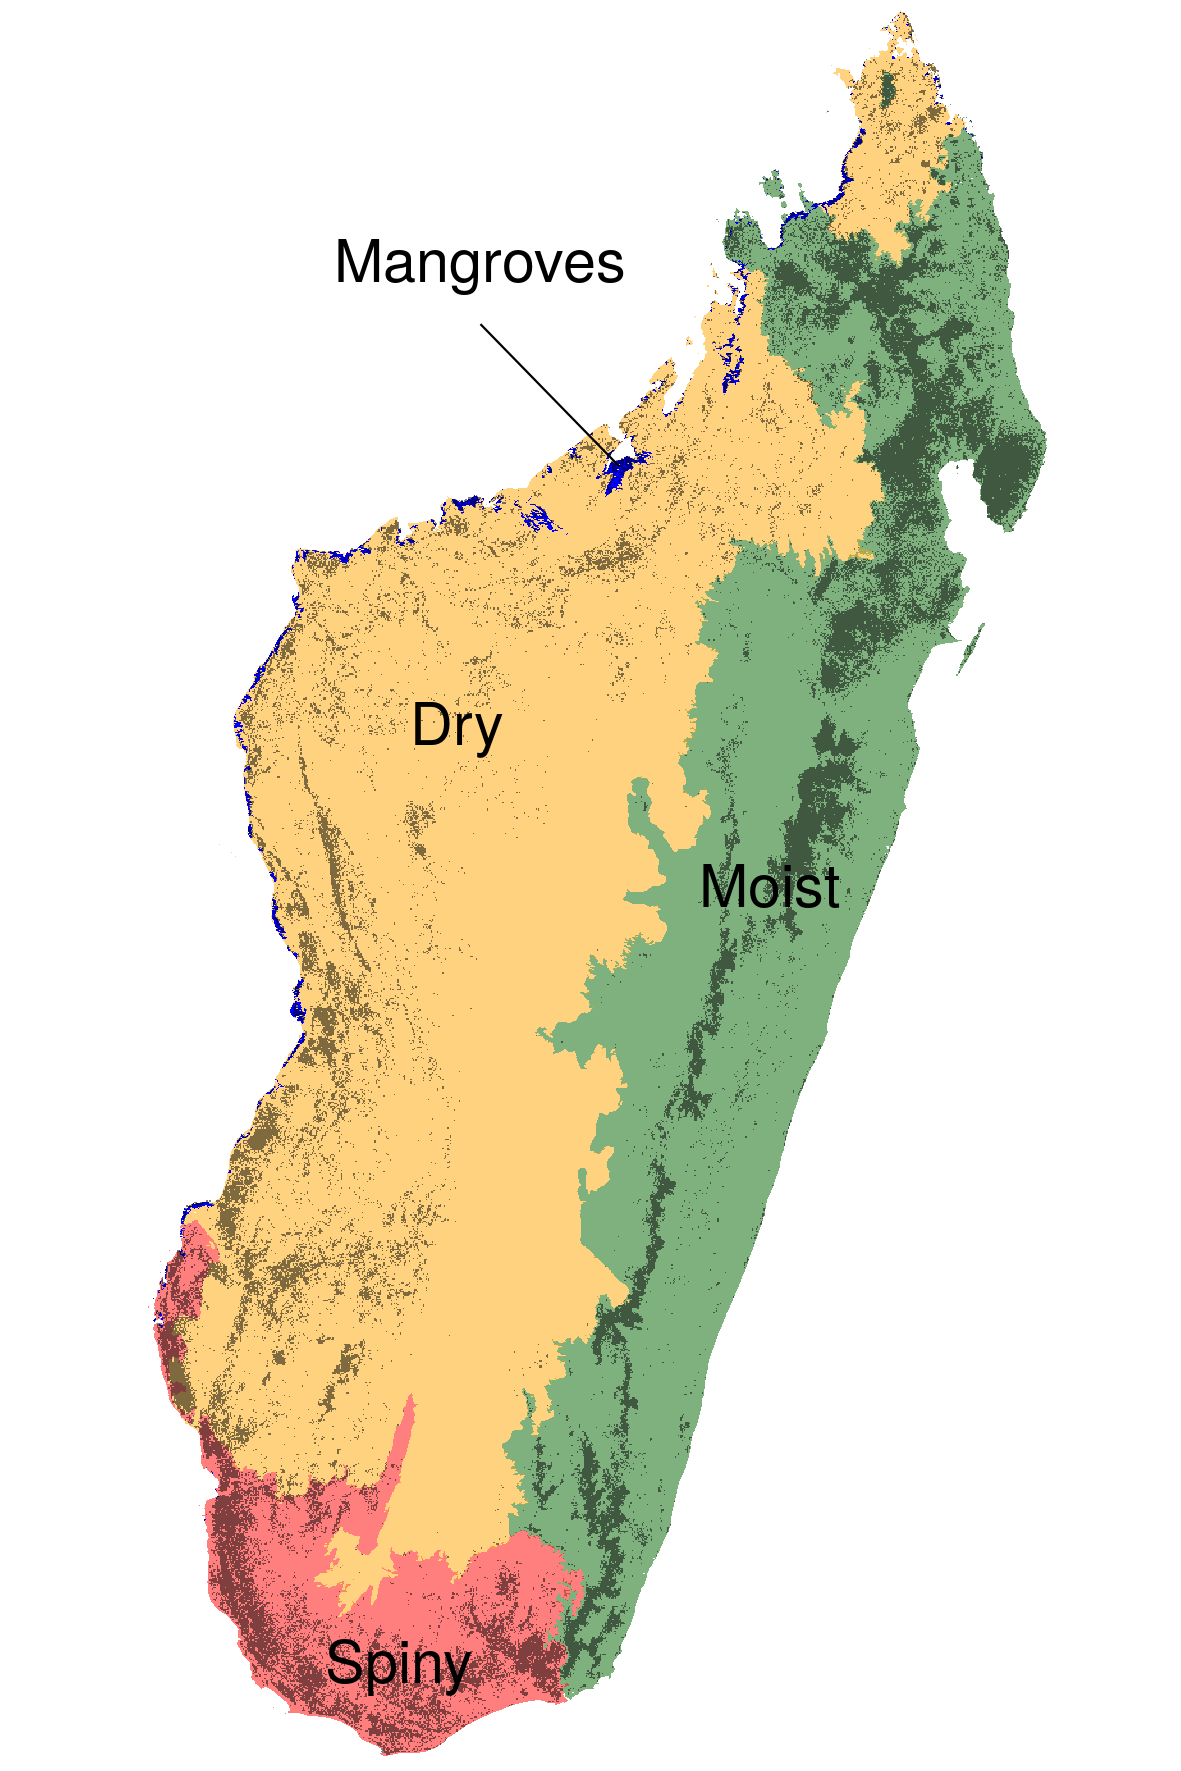
\includegraphics[width=11cm]{figs/ecoregion.png}

    \caption{\textbf{Ecoregions and forest types in Madagascar.}
      Madagascar can be divided into four climatic ecoregions with
      four forest types: the moist forest in the East (green), the dry
      forest in the West (orange), the spiny forest in the South
      (red), and the mangroves on the West coast (blue). Ecoregions
      were defined following climatic \citep{Cornet1974} and
      vegetation \citep{IEFN1996} criteria. The dark grey areas
      represent the remaining natural forest cover for the year 2014.}
   
    \label{fig:ecoregion}
    
\end{figure}
\vfill

\newpage

\vspace*{\stretch{1}}
\begin{figure}[h!]
  \centering
  
  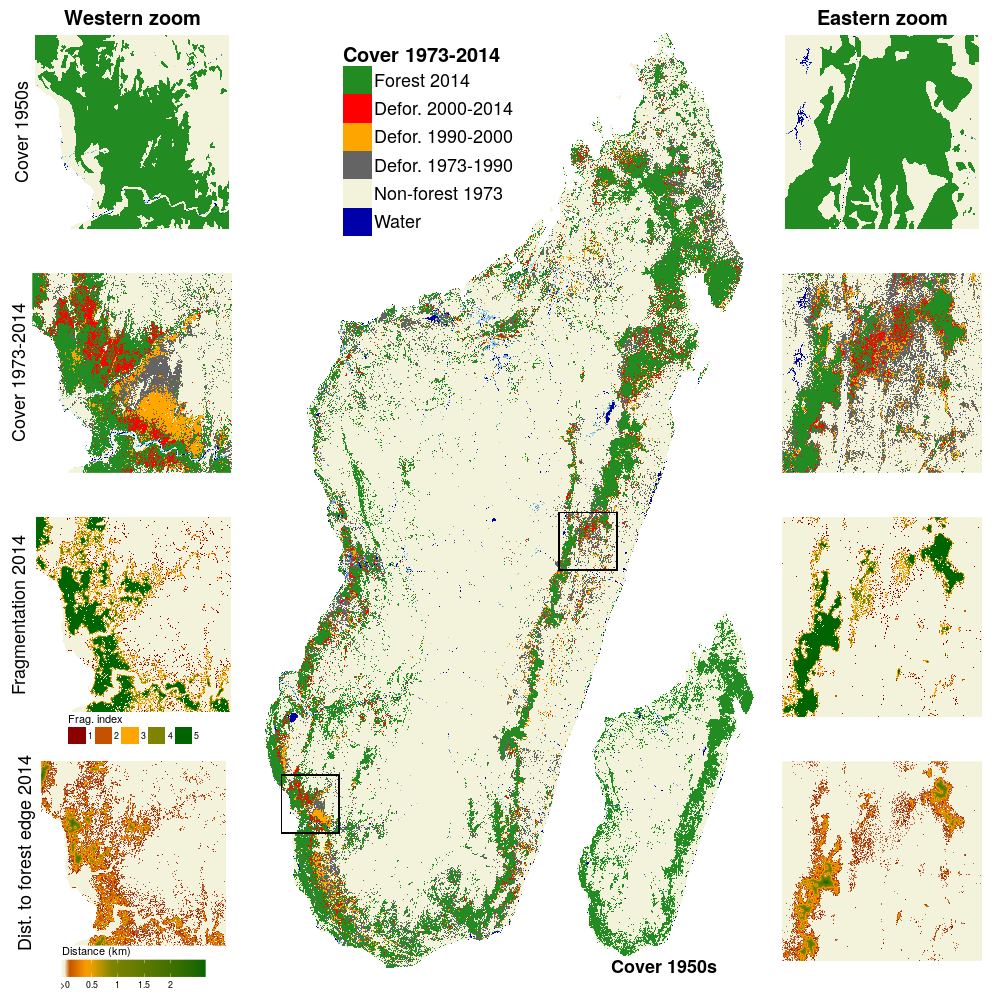
\includegraphics[width=\textwidth]{figs/fig_fcc.png}

  \caption{\textbf{Forest cover change on six decades from 1953 to
      2014 in Madagascar.} forest cover changes from \emph{c.} 1973 to
    2014 are shown in the main figure, and forest cover in \emph{c.}
    1953 is shown in the bottom-right inset. Two zooms in the western
    dry (left part) and eastern moist (right part) ecoregions present
    more detailed views of (from top to bottom): forest cover in
    1950s, forest cover change from \emph{c.} 1973 to 2014, forest
    fragmentation in 2014 and distance to forest edge in 2014. Data on
    water bodies (blue) and water seasonality (light blue for seasonal
    water to dark blue for permanent water) has been extracted from
    \citet{Pekel2016}.}

  \label{fig:fcc}

\end{figure}
\vspace*{\stretch{1}}

\newpage

\vspace*{\stretch{1}}
\begin{figure}[h!]
  \centering
  
  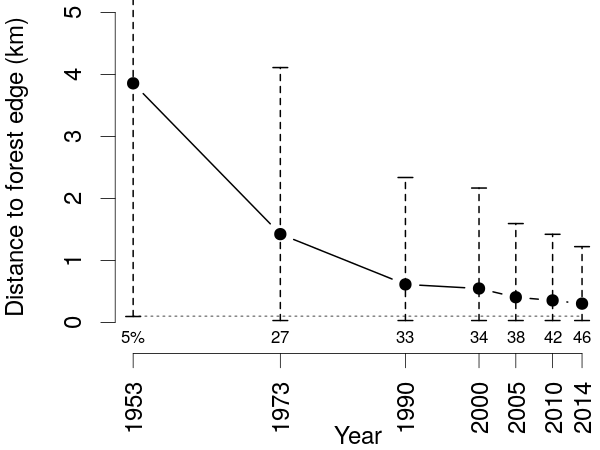
\includegraphics[width=12cm]{figs/dist.png}

  \caption{\textbf{Evolution of the distance to forest edge from 1953
      to 2014 in Madagascar.} Black dots represent the mean distance
    to forest edge for each year. Vertical dashed segments represent
    the 90\% quantiles (5\% and 95\%) of the distance to forest
    edge. Horizontal dashed grey line indicates a distance to forest
    edge of 100~m. Numbers at the bottom of each vertical segments are
    the percentage of forest at a distance to forest edge lower than
    100~m for each year.}
  
  \label{fig:dist_edge}

\end{figure}
\vspace*{\stretch{1}}

\end{document}
